\documentclass[a4paper, parskip=true, firsthead=false, fromemail=true, foldmarks=false]{scrlttr2}
\usepackage{amsmath}
\usepackage{amsfonts}
\usepackage{amssymb}
\usepackage[british]{babel}
\usepackage{kpfonts}
\usepackage{siunitx}
\usepackage[version=3]{mhchem}
\usepackage{hyperref}
\usepackage{graphicx}

\newenvironment{quotationi}
{\begin{quotation}\itshape}
{\end{quotation}}

\setkomavar{fromemail}{mathieu.leocmach@univ-lyon1.fr}
\setkomavar{signature}{Hassan Srour, Martien Duvall Deffo Ayagou, Thi Thanh-Tam Nguyen, Nicolas Taberlet, S\'{e}bastien Manneville, Chantal Andraud, Cyrille Monnereau, and Mathieu Leocmach}

\newcommand{\journal}{Soft Matter}

\begin{document}
\begin{letter}{From:\\
Mathieu Leocmach,\\
Univ Lyon,\\ 
Universit\'e Claude Bernard Lyon~1, CNRS,\\
Institut Lumi\`ere Mati\`ere,\\
F-69622, VILLEURBANNE,\\
France\\
\texttt{mathieu.leocmach@univ-lyon1.fr}
}
\opening{\bf Dear Prof. Paul Janmey,}

Thank you very much for your e-mail concerning our manuscript (SM\nobreakdash-ART\nobreakdash-09\nobreakdash-2016-002022) together with the comments of the Reviewers. 

Following the constructive comments and suggestions of the Reviewers, we have revised our manuscript. 
We believe that we have been able to answer the comments of both reviewers on a satisfactory level and thus the revised manuscript has been much improved, thanks to the valuable comments of both Reviewers. We note that the parts revised to answer the Reviewers have been highlighted with blue characters in the revised manuscript.


We hope that you and your reviewers would find that the revised manuscript is now suitable for publication in \journal. 

\closing{\bf Sincerely yours,} 
\clearpage

\textsf{\textbf{Replies to the comments of Reviewer \#1}}

\begin{quotationi}
The submitted work combines synthesis with theoretical calculation of polymer based hydrogels and is a very interesting manuscript to be published in the journal Soft Matter. The authors explain in a well-structured way their experiments and the conclusions are supported by a variety of analytical techniques. Besides synthetic work, the reader also gets an insight into the processionary model. Nevertheless, I have some suggestions that might help improving this publication:
\end{quotationi}

We are very glad to see the positive comments of the Reviewer. Below we reply to the comments of the Reviewer one by one. 


\begin{quotationi}
Page 5, Fig. 1: Br end group of the polymer POH/PBr and Nu end group in PNu+Br- is missing in the structure.
\end{quotationi}

We thank the Reviewer for spotting this omission. Actually we are not completely sure that nucleophile substitution actually takes place on a tertiary carbon, but indeed a \ce{Nu+Br-} tail group is our best guess.

\begin{quotationi}
Page 5, chapter 2.1, beginning of 1st section (polymer analysis): Why is Mw mentioned there? I suggest that Mn is presented. Was Mn calculated via monomer conversion or end group analysis via 1H NMR? Mw/Mn = 1.089 should be rounded up to 1.09.
\end{quotationi}

This is indeed a difficult question ; although most papers dealing with polymer chemistry present the molecular weight calculated by NMR as a Mn, we personally think that Mw better fits: the methodology is indeed based on the integration of repeating unit protons, and heavy chains are overexpressed in this integration. However, on the basis that (1) The NMR calculated value can anyway, strictly speaking, neither be considered as a ``pure''  Mn or Mw (2) Mn agrees better with existing literature (3) Polydispersity is anyway low, we changed the sentence to ``Mn =\SI{8300}{\dalton} from NMR, \SI{5125}{\dalton} from GPC''.

%we changed the text to give Mn instead of Mw

\begin{quotationi}
Page 5, chapter 2.1, end of 2nd section (peaks of Br-/I-, detection limits for F-/Cl-): Where do 89/91 and 121 come from? The peaks of Br- and I- should be 79/81 and 126. The content of the text does not fit to what is shown in S2 and S3.
\end{quotationi}
We thank the Reviewer for spotting this typo. We quite fortunately agree with the periodic table.

\begin{quotationi}
 It also should be found an alternative analysis method to proof the successful anion exchange for F- and Cl-.
\end{quotationi}
We think that the complete disappearance of any trace of Br- from the MS spectrum after addition of either NaCl or NaF is a clear evidence that the process occurred successfully. We initially thought of other alternative methods, namely atomic absorption  and elemental analysis: the former is no more available in our laboratories; and we know that the latter is practically really tricky on those highly hygroscopic polymers, as water tends to accumulate within the sample during either storage or preparation (as seen in the DSC spectrum) making it very difficult to get reliable data.

\begin{quotationi}
Page 6, chapter 2.2, beginning of 1st section (listing of compounds): Abbreviations can be used here for bromide, iodide 
\end{quotationi}

This is done.

\begin{quotationi}
Page 7, Fig. 4: Why are all the amplitude sweeps measured until different deformation values and not all from 10-3 till e.g. 102? What is the unit there [\%]? Further, weight percent is abbreviated as wt\%.
\end{quotationi}

As the Reviewer kindly suggested, the amplitude sweeps were programmed to run between $10^{-3}$ and $10^2$ for all samples. However the rheometer can only apply a torque larger than a minimum value to perform reliable measurements. Beyond the plastic regime, the samples are shear thinning and the rheometer always reaches its minimum torque at strain amplitudes smaller than $10^2$. Since further measurement points are not reliable we do not display them.

As it is common in the rheology literature, strains are given without units since they are non dimensional. A strain of 1 is 100\%.

\begin{quotationi}
Page 7, chapter 2.3: In the text you mention the materials are shear thinning. The amplitude sweeps shown indicate that the structure of the material is changed when leaving the linear viscoelastic region. Because both moduli are decreasing this is indicating shear thinning properties. A clear prove for shear thinning would be given using rotational experiments (viscosity over shear rate plots).
\end{quotationi}

As mentioned in the text, our samples display a strong Weissenberg effect. In our cone-plane geometry, it results in outward ejection of the sample at moderately high shear rates. To free us from Weissenberg effect we could have used a Couette geometry, but the amount of material to synthesise to fill this geometry would have been prohibitive (about 20 times the cone-plate volume).

\ce{PIm+Br-} was the most well-behaved gel by this standard and we were able to perform flow curves on a reasonable range of shear rates (see Fig 2 of our previous paper \href{http://doi.org/10.1002/marc.201400478}{Srour et al. Macromolecular Rapid Communications 2015}). Indeed viscosity drops as shear rate increases confirming our claim of shear thinning.

Qualitatively the other gels follow this trend, but the range of accessible shear rates is much more limited before Weissenberg-induced sample ejection kicks in (less than a decade for \ce{PPyr+I-}). Therefore we decided not to present flow curve data and instead show only the more reliable amplitude sweeps.



\begin{quotationi}
Page 7, chapter 2.3, beginning of 2nd section (imidazolium and pyrrolidinium based gels): Please insert here a short explanation why immidazolium based gels are much weaker than their pyrrolidinium counterpart.
\end{quotationi}

This paragraph was meant to be descriptive and not explicative. At this point in the text we do not have an explanation on why immidazolium based gels are much weaker than their pyrrolidinium counterpart or why \ce{Cl-} gives a weaker gel than \ce{Br-}. We only note that gel shear modulus follows counter-ion condensation. Explanations will come with the model. We rephrased the first sentence of the paragraph to make its purpose clearer.

\begin{quotationi}
Page 10, chapter 2.4.3: typing error (“the the correlation”)
\end{quotationi}

Fixed.

\begin{quotationi}
Supporting Information
Please insert 1H NMR spectrum of POH in order to understand the calculation of Mn.
\end{quotationi}

Thank you for the suggestion, the figure has been added as Figure S2; the caption depicts the methodology used for Dp/Mn calculation.

\begin{quotationi}
Page 2, 1st chapter (SEC analysis): Please change polydispersity index PDI to dispersity \DJ.
\end{quotationi}

Done.

\begin{quotationi}
Page 8: Weight percent is abbreviated as wt\%.
\end{quotationi}

Done.



We hope that the Reviewer would think that the revised manuscript has been much improved and is now suitable for publication in \journal. 
 
\clearpage

\textsf{\textbf{Replies to the comments of Reviewer \#2}}

First we would like to thank the reviewer for having carefully read our manuscript and provided valuable comments and suggestions.

\begin{quotationi}
The authors report on rheological characterization and theoretical interpretation of properties of polyelectrolyte assemblies prepared from molecules with a single anionic headgroup and cationic groups along the chain. The presented work including preparation of the polyelectrolytes, their rheological characterization in solution as well as theoretical interpretation, is considered to be conducted in a nice way, it indicate the role of counterions in affecting the assembly modes of the structures and novel assembly modes are suggested. There are, however, some concerns that should be addressed before publication can be recommended:

Although offering novel handles to generate molecular assemblies, and for this reason, is considered to be general interest, the suggestion for the particular structures being assembled could be further bolstered by scattering tools.
\end{quotationi}

In many instances we tried to perform DLS measurements on our samples and, indeed, signals were observed. However the obtained results were largely unreproducible (even for a given sample upon slight change of the concentration, not to mention when two different samples were used). An example is shown below.

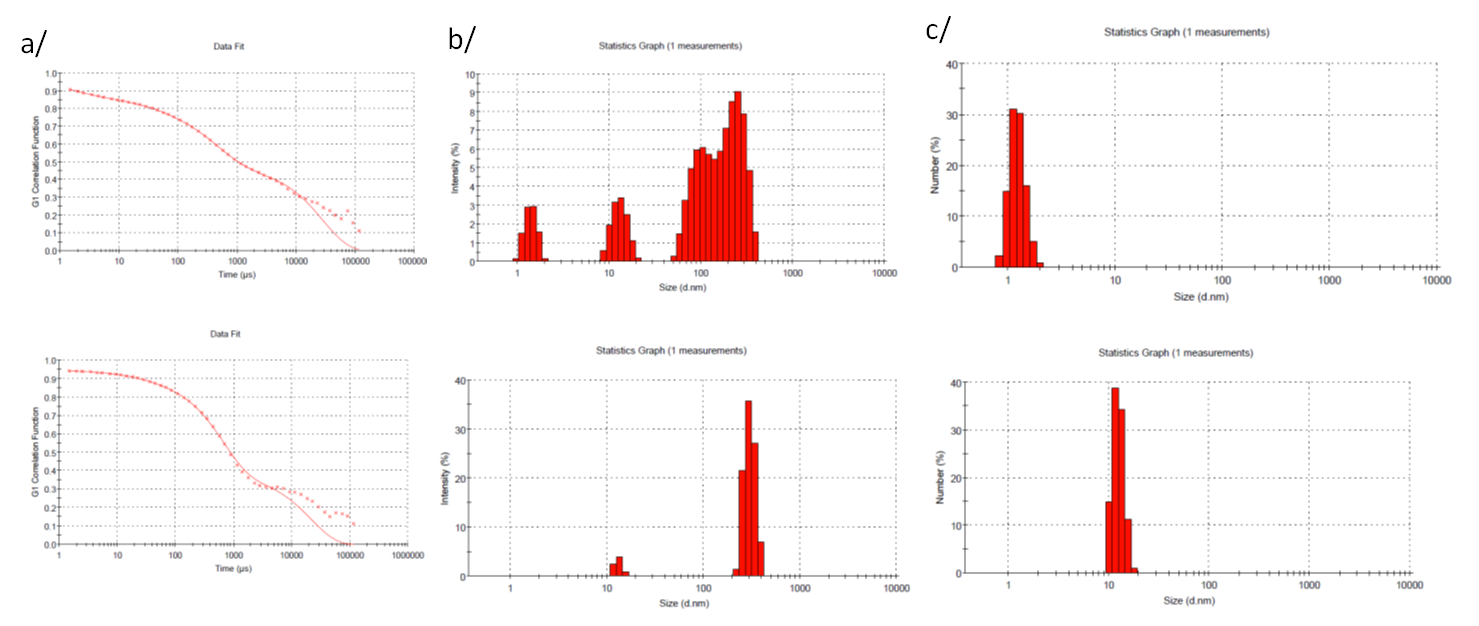
\includegraphics[width=\textwidth]{DLS.png}
\textit{Figure: \textbf{a} DLS data and best fit \textbf{b} size distribution by diffusion intensity and \textbf{c} size distribution by number for PImBr (top row) and PPyrBr (bottom row) in water at 10\% weight concentrations}

As the Reviewer can see, dispersion was very high, and signal quality so low that cumulant fit analyses were absolutely irrelevant. In our opinion, there is nothing relevant in these data, this is why we finally chose not to include it in the SI. If the referee thinks that it might be worth adding some of these data to the article, we are ready to do it. However, we do know whether a reasonable interpretation could be provided from the data. We leave the referee judge; top is PImBr bottom PPyrBr. Although a pattern seems to exist, it seems difficult to us to get its exact meaning, and to separate the artefact from the fact\ldots

\begin{quotationi}
In applying network theory to interpret the data, it appears that e.g. loose end corrections are not employed. What is the rational for that?
\end{quotationi}

To our understanding, loose end corrections describe a situation where pre-existing linear chains of size $M$ are randomly cross-linked with an average of $M_c$ monomers between cross links with $M_c\leq M/2$. The modulus then scales as
\begin{equation}
\frac{G}{k_\mathrm{B}T} = \frac{c}{M_c}  \left(1 - \frac{2M_c}{M}\right).
\end{equation}
For example if $M_c$ is only one third of $M$, then two third of the original linear chain are loose ends and do not contribute to the elasticity.

This is rather different from our situation where the number of monomers between cross links is larger or equal to the number of monomers in the original chain. This situation stems from the reactivity of the heads: a cross link necessarily occurs at the head of a polymer, preventing one of the possible loose end, but leaving the possibility of many loose ends at the tails of each polymer.

We can better compare our situation to a gel formed by branched polymers, for example bottle brush polymers. In this situation, Papagiannopoulos et al. (\href{http://doi.org/10.1021/bm060287d}{Biomacromolecules 2006} or \href{http://doi.org/10.1039/b714864j}{Faraday Discussions 2008}) have shown that the shear modulus scales as
\begin{equation}
\frac{G}{k_\mathrm{B}T} = \frac{c}{N_\mathrm{tot}}.
\end{equation}
where $N_\mathrm{tot}$ is the total number of monomers between cross-links, including side chains that are topological `loose ends'. 

In other words, one can consider two possible definitions of ``cross link''. In Flory's definition, every branching point is a cross link, therefore a brush has many loose ends. In the more coarse-grained definition used by Papagiannopoulos et al., branching points leading to a loose end are not considered meaningful cross links, but every monomer of the side chains actually contribute to entropy and thus to elasticity.

We added a paragraph at the end of 2.4.2 to stress this difference.


\begin{quotationi}
In the introduction, the authors refer to interest in hydrogels in general is related to their application potential in biomedicine, but do not explicitly relate the particular conditions used to modulate properties also to such an application domain later in the manuscript. Are the various solution conditions studied compatible with such applications? Are the results sensitive to addition of a background electrolyte (e.g., similar to physiological ionic strength)?
\end{quotationi}

We thank the Reviewer for this excellent suggestion. We added a paragraph and Figure 8b to describe the predictions of our model concerning the consequences of a background electrolyte concentration similar to physiological ionic strength. We think it demonstrates quite well the power of our model as well as the robustness of our claims concerning potential biomedical applications. However making our gels biocompatible would demand a careful selection of the ion pairs to ensure lack of toxicity, a feature that is out of the scope of the present paper.





We hope that the Reviewer would think that the revised manuscript is now suitable for publication in \journal. 


%\cc{Cclist} 
%\ps{adding a postscript} 
%\encl{list of enclosed material} 
\end{letter} 
\end{document}